\documentclass[a4paper,12pt]{article}
\usepackage[T1]{fontenc}
\usepackage{imakeidx}
\usepackage{graphicx}
%\makeindex[columns=3, title=Alphabetical Index, intoc]
\usepackage{graphicx,wrapfig,lipsum}

\begin{document}

\textbf{Daniele Della Cioppa}

\textbf{Software Developer}

\tableofcontents
\clearpage

\section{Knowledge unit}

This is what I've been covering so far during the apprenticeship:

\begin{itemize}
\item {database development}
\item {application life cycle}
\item docker
\item github 
\item LateX
\item PostgreSQL
\item Linux
\item {iOS \& Android development}
\end{itemize}
\clearpage

\subsection{iOS \& Android development}
In Figure 1 we can see the stage I was on the 23rd March, with the mobile development. The progress of the whole thing can be very slow since this is being literally self taught during my office hours \newline

\begin{wrapfigure}{r}{5cm}
\centering
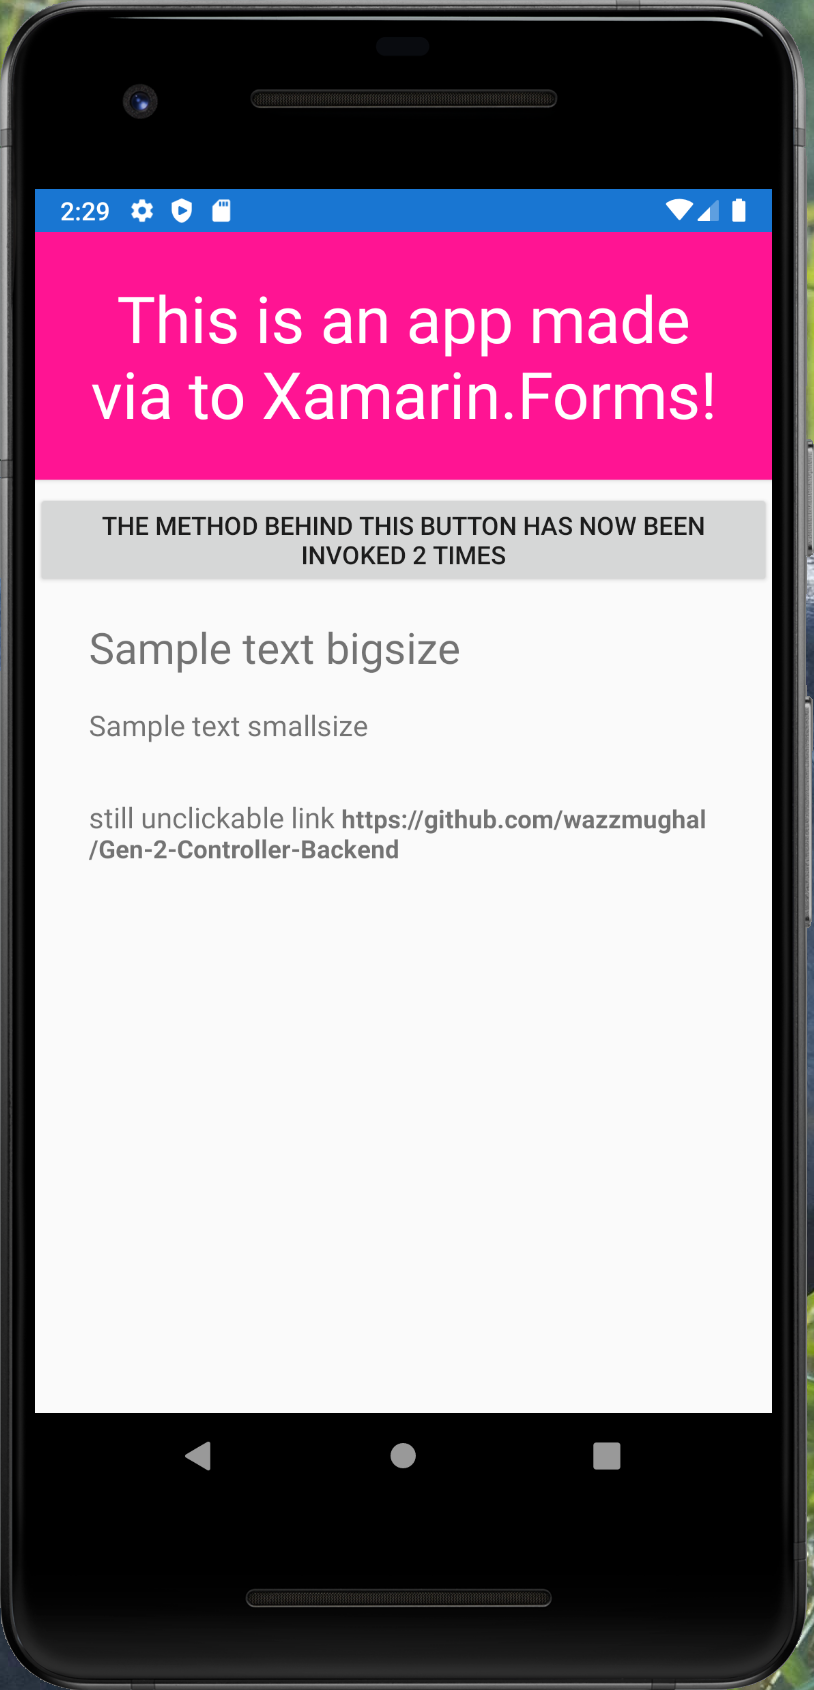
\includegraphics[width=5cm]{./capture-app.PNG}
%\vspace{-10pt}
\caption{Hello World in Xamarin with a button\footnotemark{}}\label{wrap-fig:1}
\end{wrapfigure} 

\footnotetext{the button invokes an event saying how many times the user clicked it}
\noindent We realized Xamarin brings in some difficulties even experts are struggling with. Since I'm on an apprenticeship we agreed to make it simple and use Android Studio to make an app for Android and later on use XCode for Apple. The problem with Apple is we'll need a real physical iPhone to test the app on

After a little research I found out a tool called maptiler but it was going to be sunset soon so I've had to search more and I came up with \textbf{OSMDroid}

Figure .2 shows how the app looks now on a Motorola g7. Some functionalities have been added to test separately Client and Server functions. My app needs to interact with a C++ Server but because of the burden it takes to switch the real server on I've developed a quick server to have tests with and then once in a while see how it goes with the real server when it gets turned on.

\subsubsection{targets set on the 5th May 2022}

\begin{itemize}
\item{Login activity}
\item{nice user interface}
\item{heavy testing against bugs}
\item{calculation of middle position of all streetlight and having the map to start centered on that position}
\item{iOS instance}
\end{itemize}

\clearpage

\subsection{Stage I was at on the 5th May 2022}

\begin{wrapfigure}{r}{5cm}
\centering
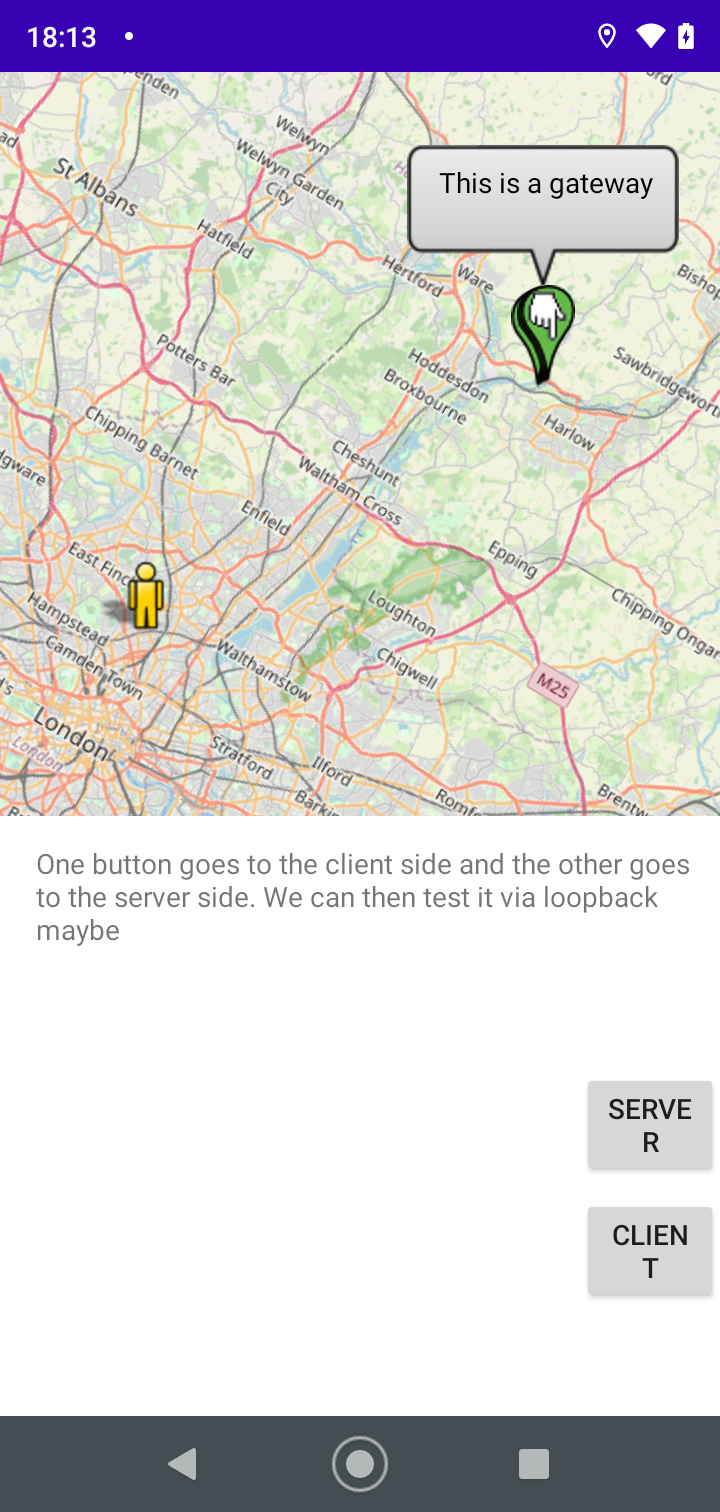
\includegraphics[width=4cm]{./current_status_g7.PNG}
%\vspace{-10pt}
\caption{User Interface on a Motorola g7}\label{wrap-fig:2}
\end{wrapfigure}

\begin{wrapfigure}{r}{5cm}
%\centering
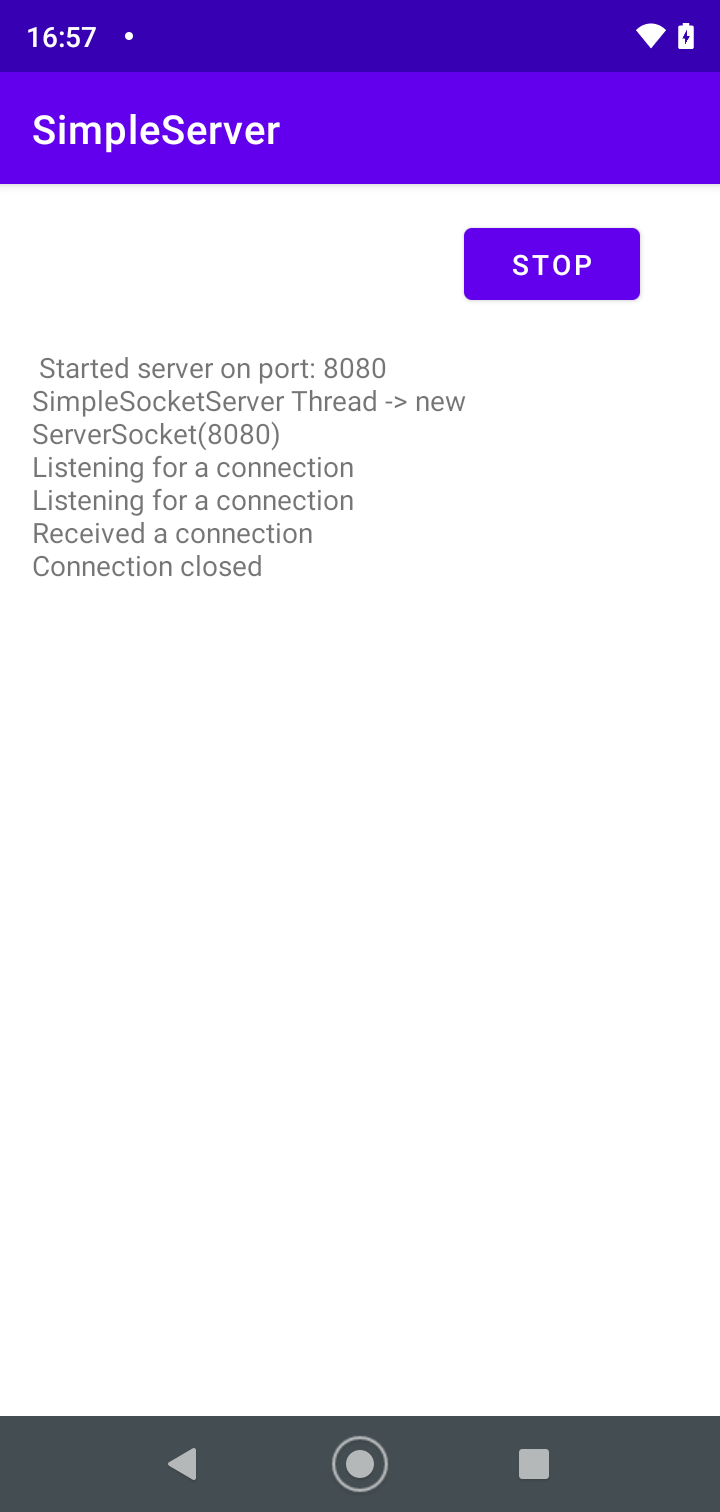
\includegraphics[width=4cm]{./server_g7.PNG}
%\vspace{-10pt}
\caption{server activity on a Motorola g7}\label{wrap-fig:3}
\end{wrapfigure}

\begin{wrapfigure}{r}{5cm}
%\centering
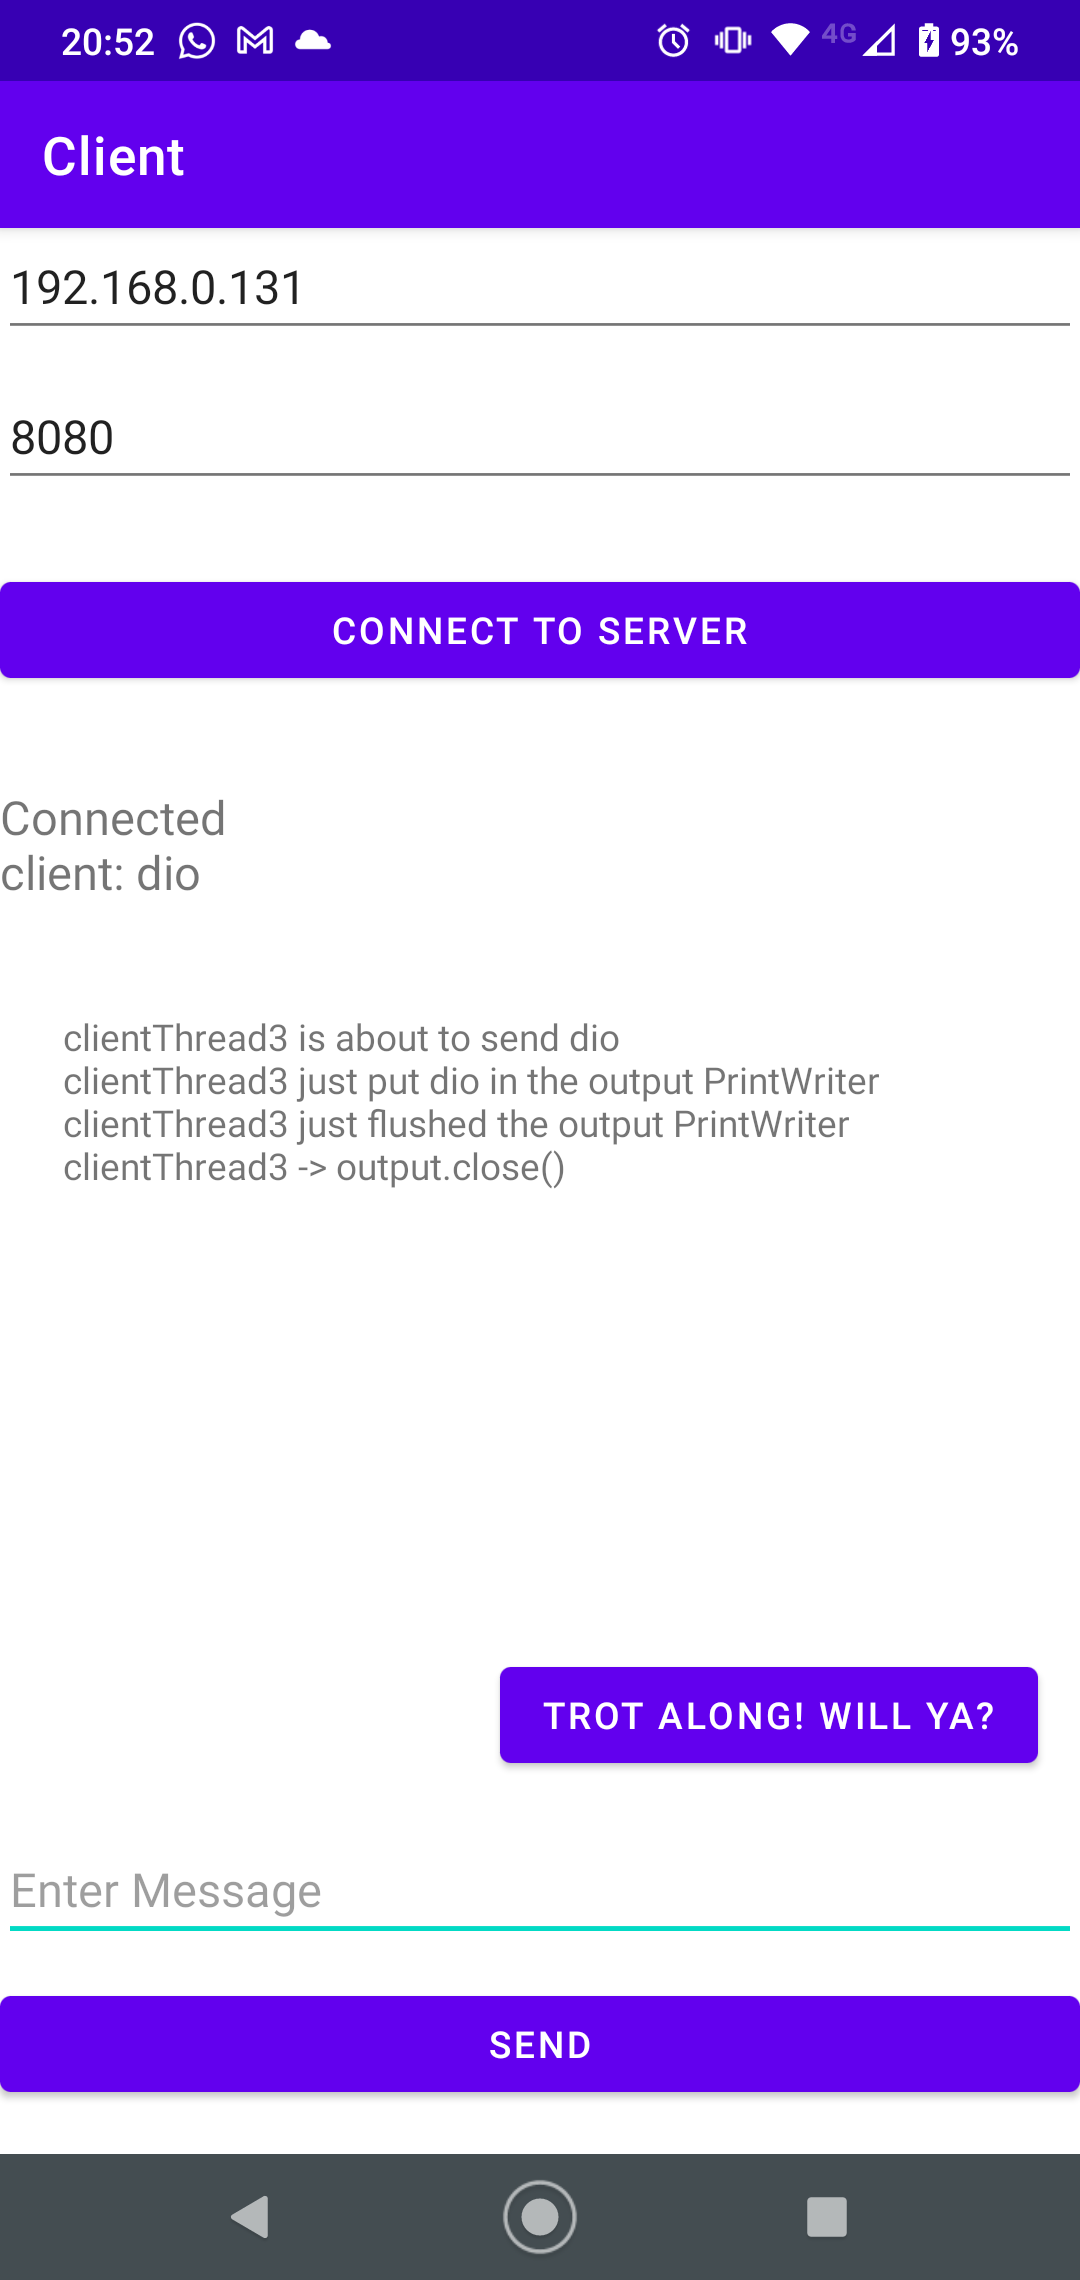
\includegraphics[width=4cm]{./client_g8.PNG}
%\vspace{-10pt}
\caption{client activity on a Motorola g8}\label{wrap-fig:4}
\end{wrapfigure}


\begin{wrapfigure}{r}{5cm}
%\centering
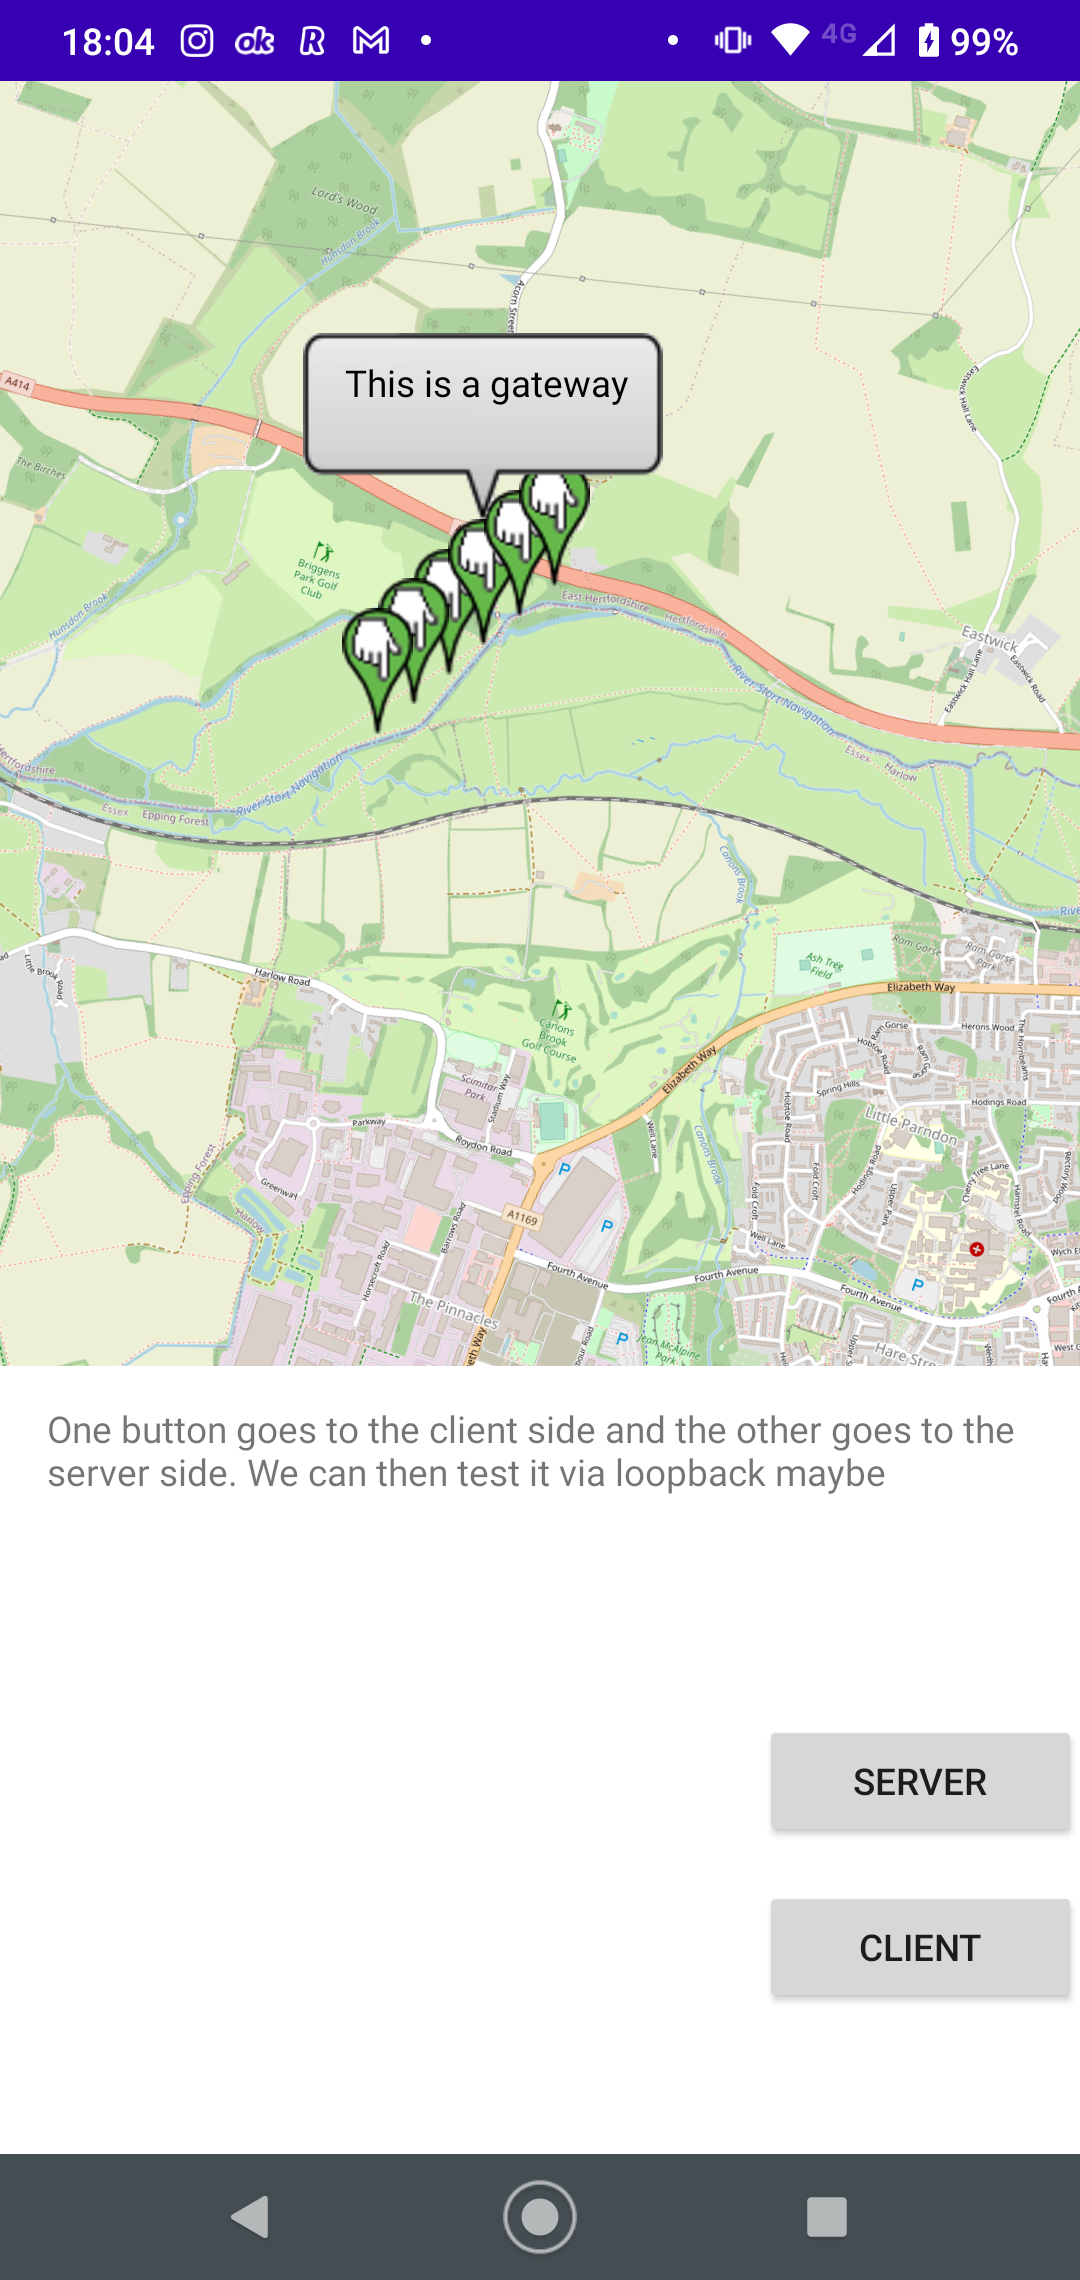
\includegraphics[width=3cm]{./current_status_g8.PNG}
%\vspace{-10pt}
\caption{User Interface on a Motorola g8}\label{wrap-fig:4}
\end{wrapfigure}


In Figure .2 you can find the stage I was at on the 5th of May where we're experimenting having the client and the server to talk to each other. The functionality it's still incapsulated in the client and needs to become part of the app rather than an external button. Figure .3 shows how is the server activity doing on a Motorola while the client (Figure .4) being run on a Motorola g8 attempts a connection to the server









\section{My Responsibilites}

After three months in my role I'm now responsible for the following tasks with databases:

\begin{itemize}
\item {reading the specs}
\item design
\item implementation
\item testing 
\item documenting
\end{itemize}

\clearpage

\subsection{design}
This is a first idea of the database I came up with

\noindent \includegraphics[width=14cm]{./ERSchemaGen2.jpg}

We agreed it was holding probably more information than what we need to display in the app so I came up later on with a smaller design which really has just the right amount of things we need to make sure we can run enough tests and see how the App, the Server and the Database interact between each other
\clearpage

This is the smaller database designed again from scratch. We need to add geolocation to nodes but for the time being it will be hard coded in the server and we'll try to see if we can display a hardcoded geolocation hold by the server to be caught by the client and displayed properly on the app

\noindent 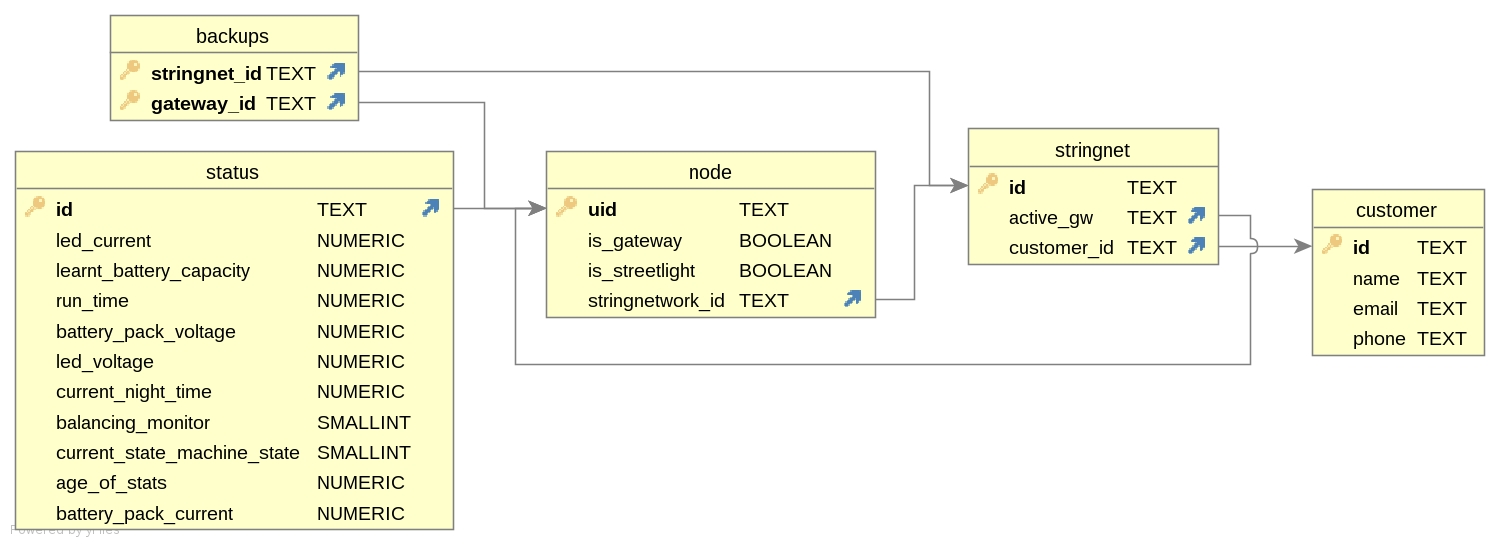
\includegraphics[width=14cm]{./SecondERSchemaGen2.jpg}

\printindex

\end{document}
